\documentclass[12pt]{article}

% Packages
\usepackage{titlesec}
\usepackage{graphicx}
\usepackage{subcaption}
\usepackage{amsmath}
\usepackage{amsfonts}
\usepackage{amssymb}
\usepackage{hyperref}

% Page layout
\usepackage[top=1in, bottom=1in, left=1in, right=1in]{geometry}

%% Title formatting
%\titleformat{\section}{\normalfont\Large\bfseries}{\thesection}{1em}{}
%\titleformat{\subsection}{\normalfont\large\bfseries}{\thesubsection}{1em}{}
%\titleformat{\subsubsection}{\normalfont\normalsize\bfseries}{\thesubsubsection}{1em}{}

% Title, author, date
\title{Report-Challenge 1}
\author{Da Vinchie Lisa, Pettenà Piero}
\date{\today} % or specify a specific date

\begin{document}

\maketitle

% Abstract if needed
% \begin{abstract}
% Your abstract goes here.
% \end{abstract}

% Table of Contents
\tableofcontents

% Start of the content
\section{Introduction}
In this challenge, our goal is to find an effective method to classify the images of the *FashionMNIST* dataset, based on their content. The dataset is formed by black-and-white images of 28 $\times$ 28 pixel, each one representing a clothing item belonging to one of the following 10 cathegories:

\begin{enumerate}
	\item T-shirt or top
	\item Trouser
	\item Pullover
	\item Dress
	\item Coat
	\item Sandal
	\item Shirt
	\item Sneaker
	\item Bag
	\item Ankle boot
\end{enumerate}

\section{Exercise 1}
The goal of this exercise is to perform Principal Component Analysis (PCA) in order to find out how the clusters are separated. In order to do that, we performed two kinds of PCA: linear and kernel PCA; then, we plotted the first two and three principal components, along with the true labels.\newline
We started by using a linear PCA, obtaining the clustering in Figure \ref{fig:pca_linear}; although the datapoints appear to be grouped in clusters, it is clear how they are not well separated; moreover, it happens that some classes have datapoints that are very far from the centroid of the cluster, as happens for class 0.
\begin{figure}[h]
	\begin{subfigure}{0.5\textwidth}
		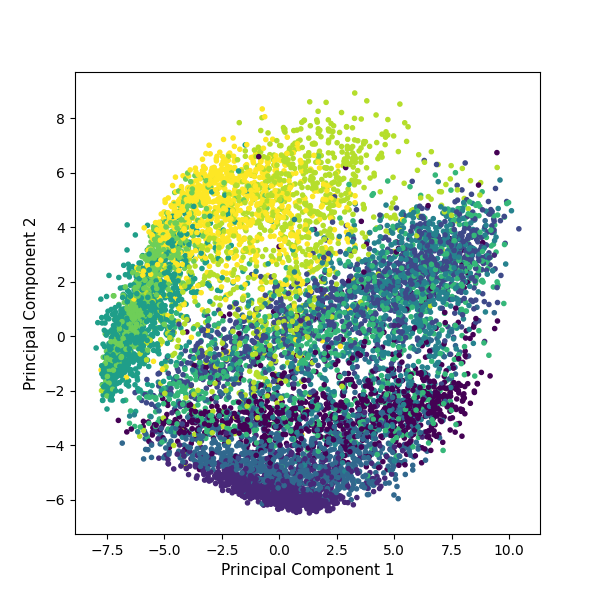
\includegraphics[width=0.4\textheight]{pca_linear_2comps.png}
		\caption{}
		\label{subfig:pca_linear_2comps}
	\end{subfigure}
	\begin{subfigure}{0.5\textwidth}
		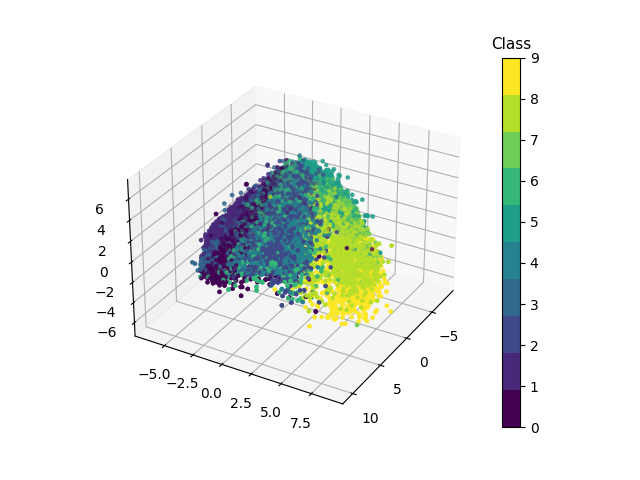
\includegraphics[width=0.4\textheight]{pca_linear_3comps.png}
		\caption{}
		\label{subfig:lpca_linear_3comps}
	\end{subfigure}
	\caption{First two and three principal components obtained by performing linear PCA, plotted along with true labels}
	\label{fig:pca_linear}
\end{figure}

Performing Kernel PCA with a Radial Basis Function kernel, using the default value of the dispersion parameter %is gamma the dispersion parameter?
 $\gamma = 1/\mathrm{\# samples} = 1/784$ , does not lead to better results, since the classes are still very mixed up, as we can see in Figure \ref{fig:pca_rbf}.
 
\begin{figure}[h]
	\begin{subfigure}{0.5\textwidth}
		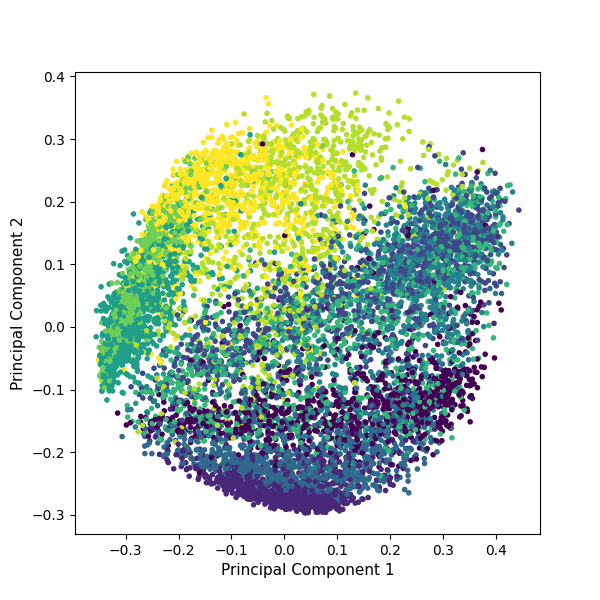
\includegraphics[width=0.4\textheight]{pca_rbf_2comps.png}
		\caption{}
		\label{subfig:pca_rbf_2comps}
	\end{subfigure}
	\begin{subfigure}{0.5\textwidth}
		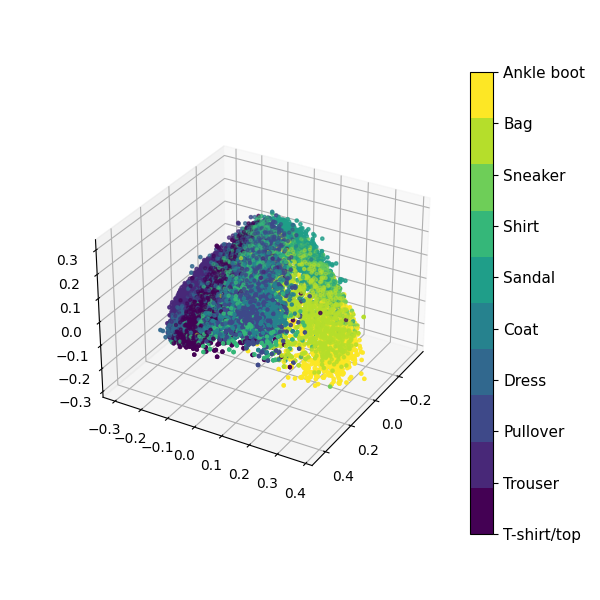
\includegraphics[width=0.4\textheight]{pca_rbf_3comps.png}
		\caption{}
		\label{subfig:pca_rbf_3comps}
	\end{subfigure}
	\caption{First two and three principal components obtained by performing kernel PCA with RBF kernel, plotted along with true labels}
	\label{fig:pca_rbf}
\end{figure}
%% Talk about parameter tuning
We tried to do the same with the polynomial and sigmoid kernels, as shown in Figure \ref{fig:pca_poly_sigmoid}, the  but none of them separates clearly the clusters. In particular, looking at the three-components plots,  it seems that datapoints with labels \textit{Ankle boot}, \textit{Bag}, \textit{Shirt}  and \textit{T-Shirt/Top} are easyer to separate, while the others are mixed up.
\begin{figure}[h]
	\begin{subfigure}{0.5\textwidth}
		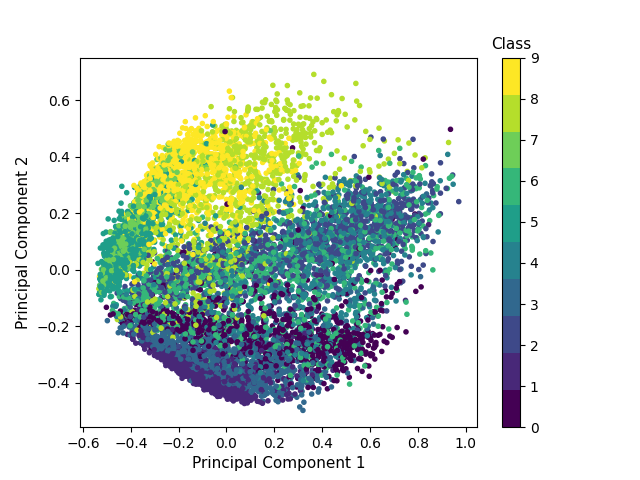
\includegraphics[width=0.4\textheight]{pca_poly_2comps.png}
		\caption{}
		\label{subfig:pca_poly_2comps}
	\end{subfigure}
	\begin{subfigure}{0.5\textwidth}
		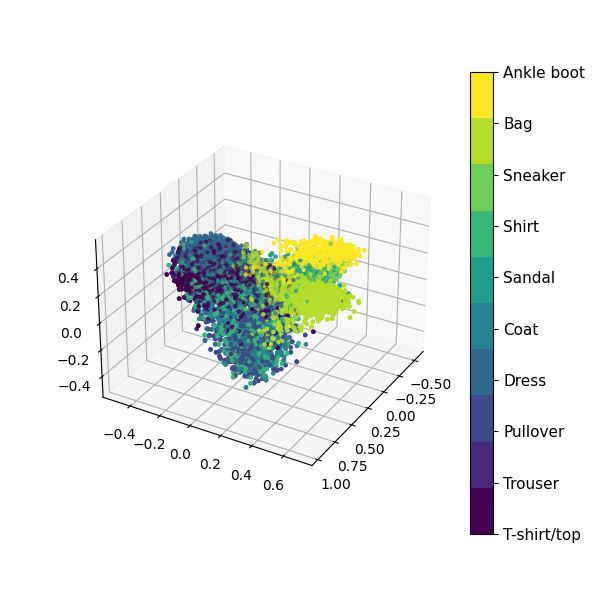
\includegraphics[width=0.4\textheight]{pca_poly_3comps.png}
		\caption{}
		\label{subfig:pca_poly_3comps}
	\end{subfigure}
	\begin{subfigure}{0.5\textwidth}
		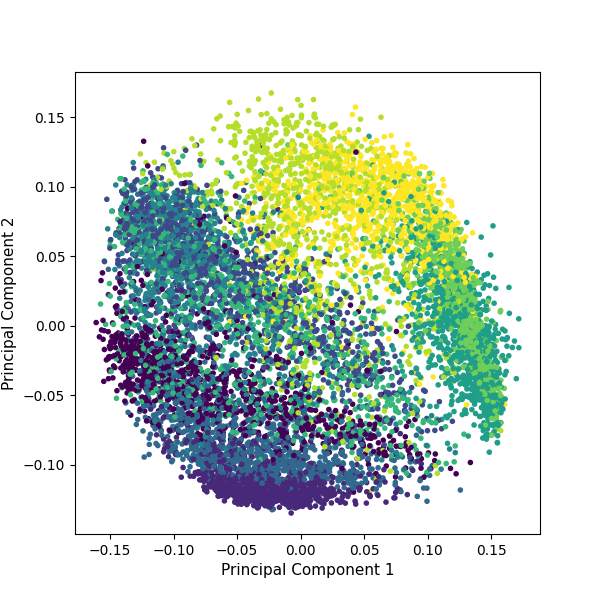
\includegraphics[width=0.4\textheight]{pca_sigmoid_2comps.png}
		\caption{}
		\label{subfig:pca_sigmoid_2comps}
	\end{subfigure}
	\begin{subfigure}{0.5\textwidth}
		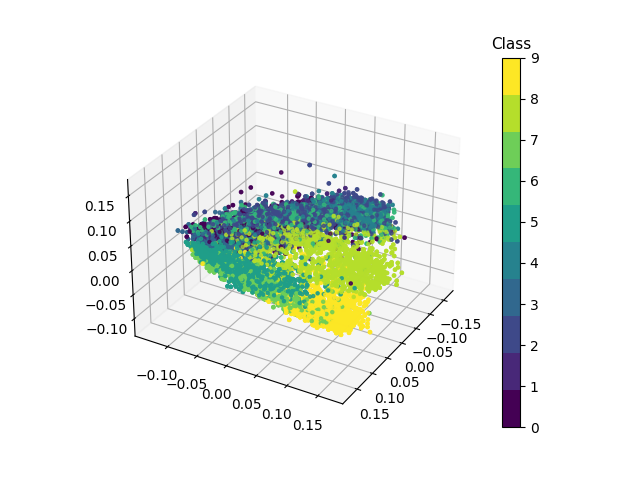
\includegraphics[width=0.4\textheight]{pca_sigmoid_3comps.png}
		\caption{}
		\label{subfig:pca_sigmoid_3comps}
	\end{subfigure}
	\caption{First two and three principal components obtained by performing kernel PCA with polynomial ((\subref{subfig:pca_poly_2comps}) and (\subref{subfig:pca_poly_3comps})) and sigmoid  ((\subref{subfig:pca_sigmoid_2comps}) and (\subref{subfig:pca_sigmoid_3comps})) kernel, plotted along with true labels.}
	\label{fig:pca_poly_sigmoid}
\end{figure}


\section{Exercise 2}
Even though no PCA method separates the datapoints in a satisfying way, we decided that the kernel PCA with sigmoid kernel is the one that works better. Then, we performed unsupervised clustering on those data, using three methods: K-means clustering, spectral clustering and Gaussian Mixture, obtaining the results showed in Figure \ref{fig:unsupervised_clustering}.\newline
\begin{figure}[h]
	\centering
	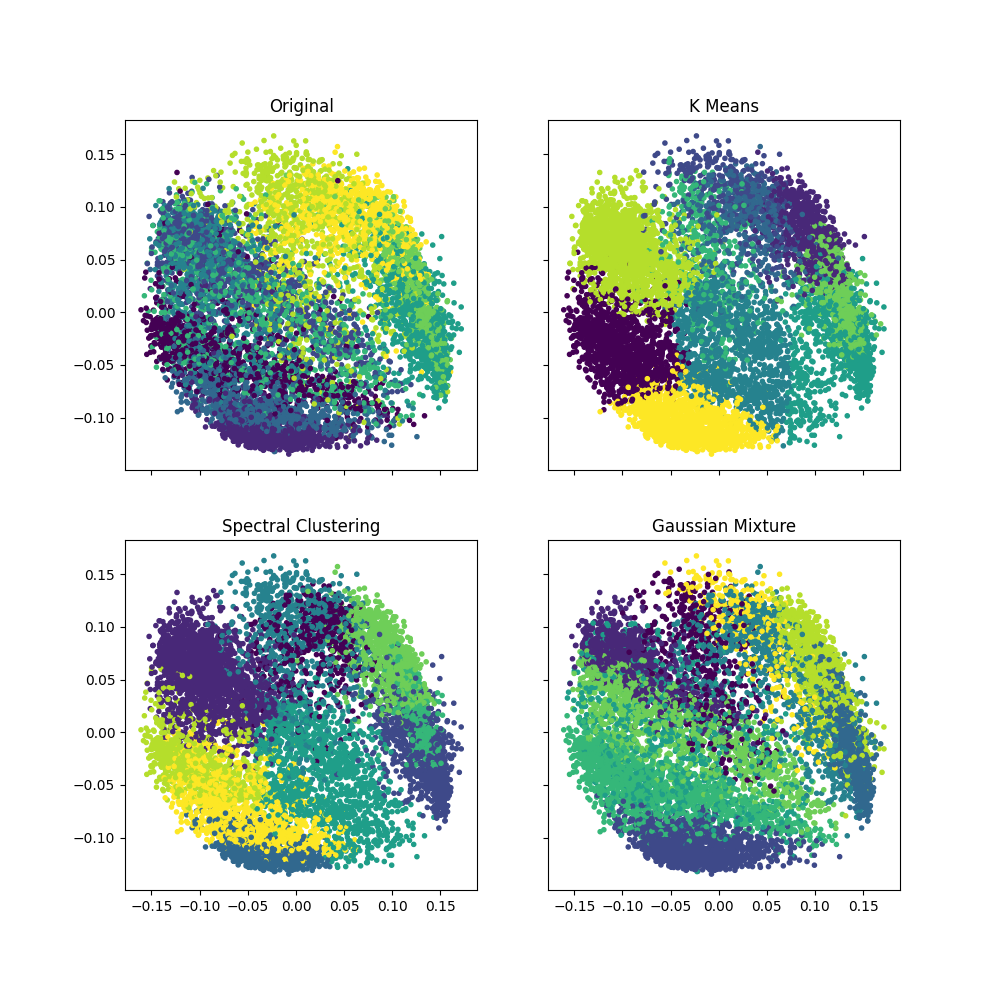
\includegraphics[width = 1 \textwidth]{unsupervised_clustering.png}
	\caption{Unsupervised clustering obtained using K-means clustering, spectral clustering and gaussian mixture, confronted with the true labels.}
	\label{fig:unsupervised_clustering}
\end{figure}
Trying to confront the obtained results with the original labels using an accuracy score is useless, since the names of the clusters will differ. In order to provide a quantitative measure of similarity, we decided to use the \textit{adjusted rand index}: this method computes a similarity measure between two clusterings by considering all pairs of samples and counting pairs that are assigned in the same or different clusters, in the predicted and true clusterings. It has values that range between 0 and 1, with 1 meaning that the two clusters are exactly the same.\newline
The results that we obtained are the following:
\begin{itemize}
	\item K-means: 0.3628
	\item Spectral clustering: 0.4342
	\item Gaussian mixture: 0.3794
\end{itemize}
As we expected, the clusters that we found using unsupervised learnign do not resemble much the ones formed by the true labels.\newline
This, probably, is due to the fact that the clusters are not clearly separable in the first place, and that maybe 10 clusters are too many: by looking at the eigenvalues of each principal component in Figure \ref{fig:eigenvalues_sigmoid}, we can see how the knee-point is clearly on the third component.
\begin{figure}[h]
	\centering
	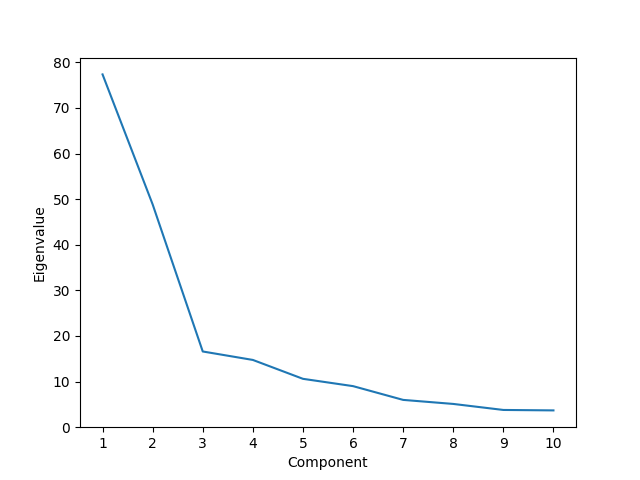
\includegraphics[width = 0.7 \textwidth]{eigenvalues_sigmoid.png}
	\caption{First 10 eigenvalues obtained by performing kernel PCA with sigmoid kernel.}
	\label{fig:eigenvalues_sigmoid}
\end{figure}


\section{Exercise 3}
In this exercise, we have to perform supervised classification, using the original images associated with one of the label sets found in the previous exercise; since the clustering made with the spectral method scored the highest rand inex, we decided to use this set of labels.\newline
To perform supervised classification, we used 3 different methods:
\begin{itemize}
	\item SVM, with different kernels;
	\item Fully Connected Neural Network;
	\item Convolutional Neural Network.
\end{itemize}
In all the three cases, we splitted our 10000 rows dataset into a train test, of 7000 rows, and a test set, of 3000 rows; this is necessary in order to evaluate the generality of the model.

\subsection{Support Vector Machine}
We performed this kind of supervised classification using the four kernels that we used for the PCA in the first exercise: linear, RBF, polynomial and sigmoid. The accuracy scores that we obtained with each kernel are the followings:
\begin{itemize}
	\item Linear: 0.9657
	\item RBF: 0.9733
	\item Polynomial: 0.9617
	\item Sigmoid: 0.3453 
\end{itemize}
%% Come mai il sigmoid kernel è quello con l'accuratezza minore, anche se abbiamo scelto proprio il sigmoid kernel nel primo esercizio?

\subsection{Fully Connected Neural Network}
We started by considering a simple neural network, with just 1 fully connected layer and a Softmax activation function; we trained it for different numbers of epochs between 0 and 20, using stochastic gradiend descent with learning rate 0.01 as the optimizer, anc aclculated the test accuracy using the cross entropy loss. As expected, the test accuracy increases with the number of epochs, as illustrated in Figure \ref{subfig:FCNN1l_accuracy-epochs}.\newline
We, then, tried a sligtly more complex neural network, with two fully connected layers and, again, the softmax activation function; in this case, we also need to choose the number of neurons of the first %penso sia il primo
layer, along with the number of neurons. We started by choosing a number of neurons of 850 and study how the accuracy grows with the number of epochs; as in Figure \ref{subfig:FCNN2l_accuracy-epochs}, we can see how we obtain better results than in the previous model.\newline
\begin{figure}
	\begin{subfigure}{0.6\textwidth}
		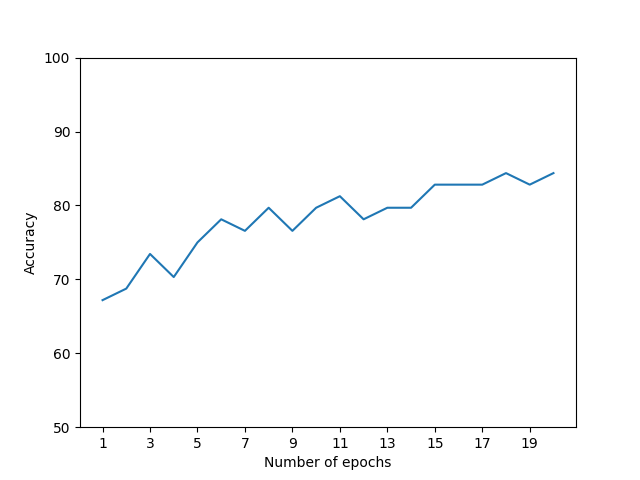
\includegraphics[width = 0.9\textwidth]{ex3_FCNN1l_accuracy-epochs.png}
		\caption{}
		\label{subfig:FCNN1l_accuracy-epochs}
	\end{subfigure}
	\begin{subfigure}{0.6\textwidth}
		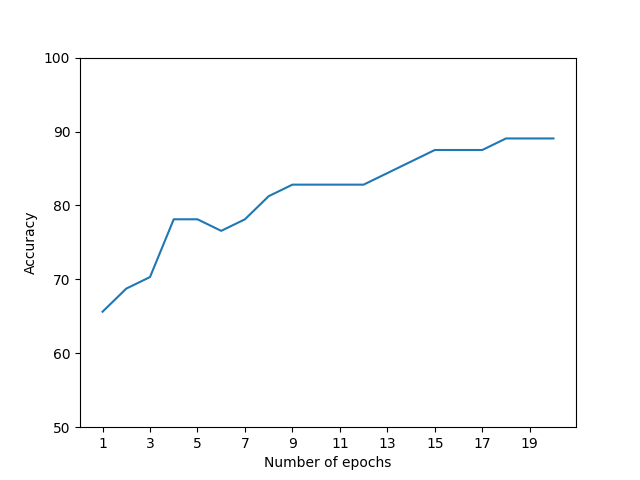
\includegraphics[width = 0.9\textwidth]{ex3_FCNN2l_accuracy-epochs.png}
		\caption{}
		\label{subfig:FCNN2l_accuracy-epochs}
	\end{subfigure}
	\caption{}
	\label{fig:ex3_FCNN_epochs}
\end{figure}

Fixing the number of epochs to 8 and changing the number of neurons between 50 and 6850, instead we obtaon the plot in Figure \ref{fig:ex3_FCNN_neurons}; here, the accuracy increases very slowly with the number of neurons.
\begin{figure}
	\centering
	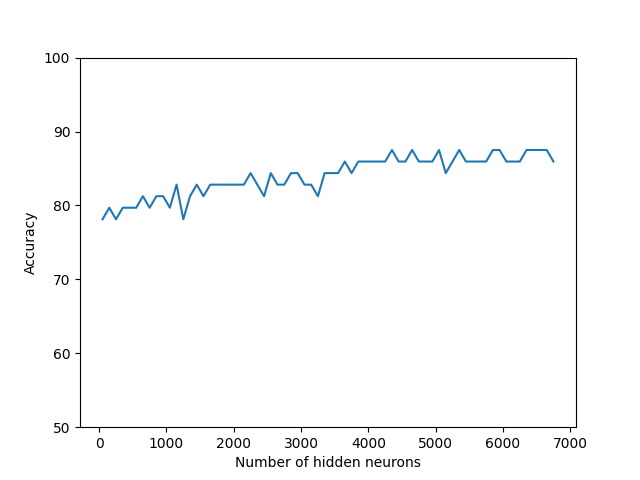
\includegraphics[width = 0.9\textwidth]{ex3_FCNN2l_accuracy-neurons.png}
	\caption{}
	\label{fig:ex3_FCNN_neurons}
\end{figure}
In conclusion, we can say that using two fully connected layers seems better than using just one; concerning the number of epochs and neurons, it seems better to prioritize the first one.

\subsection{Convolutional Neural Network}


\section{Results}
% Your content goes here

\section{Conclusion}
% Your content goes here

% References if needed
% \bibliographystyle{plain}
% \bibliography{your_bibliography_file}

\end{document}
